% \begin{figure}
%     \centering
%     \includegraphics[width=0.5\linewidth]{}
%     \caption{Caption}
%     \label{fig:enter-label}
% \end{figure}
% \begin{figure}
%     \centering
%     \fbox{\phantom{\rule{\linewidth}{1.0\linewidth}}}
%     \caption{\structeval evaluates the LLM's capability to generate structured outputs, including text-only tasks like JSON, TOML, etc, and visual rendering tasks like HTML, React, Latex, etc.}
%     \label{fig:enter-label}
% \end{figure}

\begin{figure}[t]
    \centering
    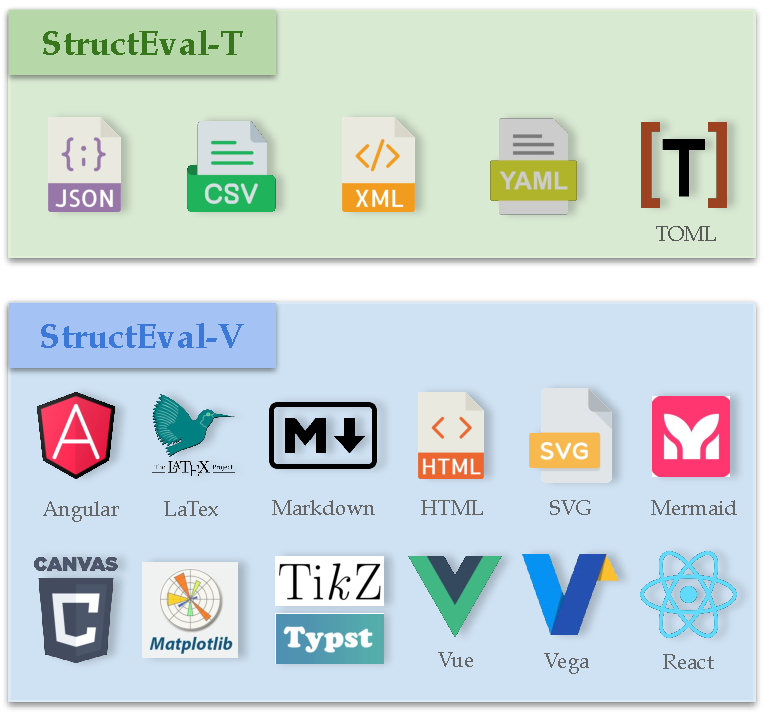
\includegraphics[width=0.98\linewidth]{./figures/intro.pdf}
    \caption{\structeval evaluates the LLM's capability to generate structured outputs, including text-only tasks like JSON, TOML, etc, and visual rendering tasks like HTML, React, Latex, etc.}
    \label{fig:intro}
\end{figure}